\section{Resultados}


\newread\tmp
\openin\tmp=../exp/shopping.entropy
\read\tmp to \ShoppingAEntropy
\closein\tmp

\openin\tmp=../exp/starbucks.entropy
\read\tmp to \StarbucksEntropy
\closein\tmp

\openin\tmp=../exp/wired_lan.entropy
\read\tmp to \WiredLanEntropy
\closein\tmp

\subsection{Escenario 1 (Red cableada)}

\begin{tikzpicture}[baseline]
    \begin{axis}[
            title={},
            xlabel={Símbolo (Dirección IP)},
            ylabel={Cantidad de información},
            scaled x ticks=false,
            scaled y ticks=false,
            width=0.45\textwidth,
            height=0.35\textwidth,
            legend pos=outer north east,
            legend cell align=left,
            ymin=0,
            xtick=data,
            xticklabels from table={../exp/wired_lan.information}{IP},
            x tick label style={rotate=80,anchor=east,font=\small}
        ]
        \addplot [ybar, fill=blue!10, draw=blue] table[x=X-Pos,y=Information]
                {../exp/wired_lan.information};

        \coordinate (A) at (axis cs:0,\WiredLanEntropy);
        \coordinate (O1) at (rel axis cs:0,0);
        \coordinate (O2) at (rel axis cs:1,0);

        \draw [blue, thick] (A -| O1) -- (A -| O2);

    \end{axis}
\end{tikzpicture}

\begin{figure}[H]
	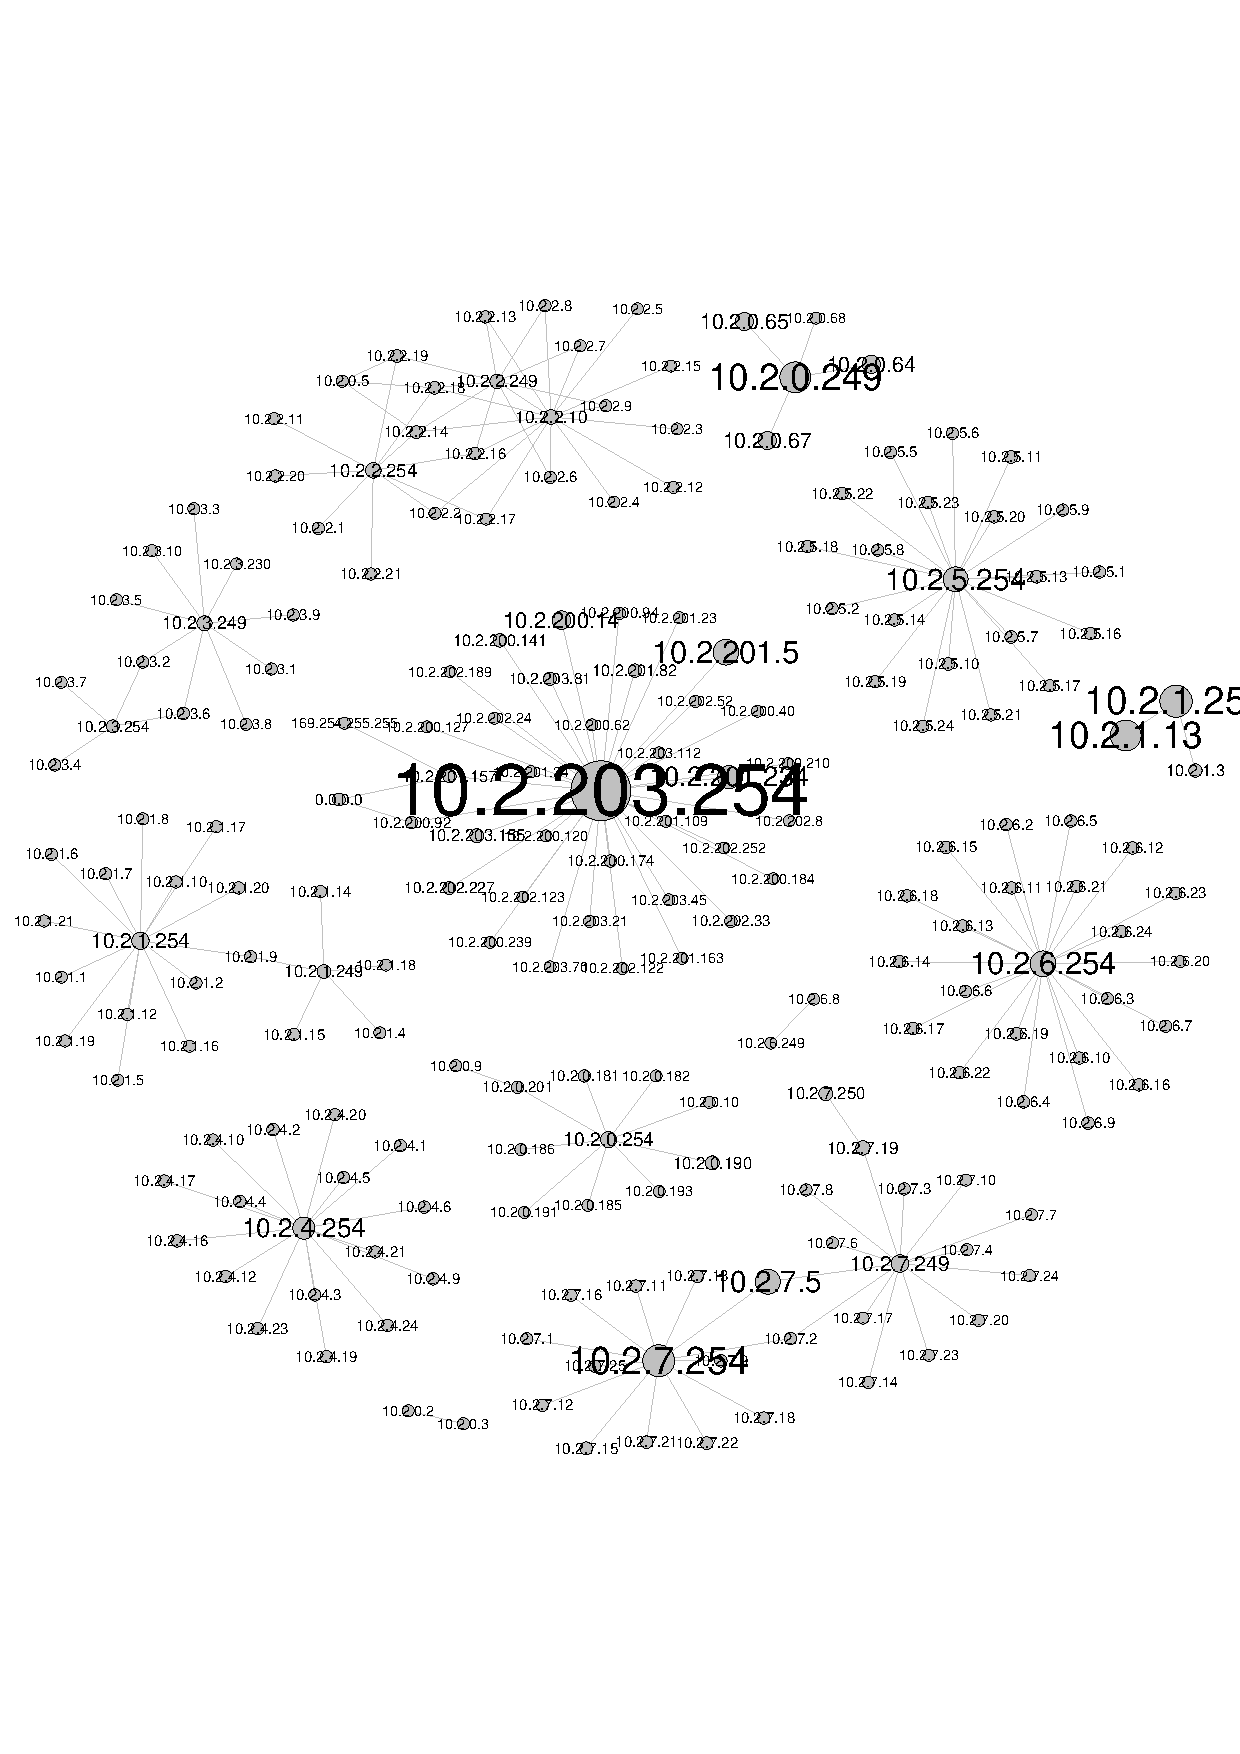
\includegraphics[scale=0.4]{figures/wired_lan.pdf}
	\caption{Red de mensajes \texttt{ARP} para captura de red cableada.}
\end{figure}

\subsection{Escenario 2 (\emph{Shopping})}

\begin{tikzpicture}[baseline]
    \begin{axis}[
            title={},
            xlabel={Símbolo (Dirección IP)},
            ylabel={Cantidad de información},
            scaled x ticks=false,
            scaled y ticks=false,
            width=0.45\textwidth,
            height=0.35\textwidth,
            legend pos=outer north east,
            legend cell align=left,
            ymin=0,
            xtick=data,
            xticklabels from table={../exp/shopping.information}{IP},
            x tick label style={rotate=80,anchor=east,font=\small}
        ]
        \addplot [
            ybar,
            fill=blue!10,
            draw=blue]
            table[x=X-Pos,y=Information]{../exp/shopping.information};

        \coordinate (A) at (axis cs:0,\ShoppingAEntropy);
        \coordinate (O1) at (rel axis cs:0,0);
        \coordinate (O2) at (rel axis cs:1,0);

        \draw [blue, thick] (A -| O1) -- (A -| O2);

    \end{axis}
\end{tikzpicture}

\begin{figure}[H]
	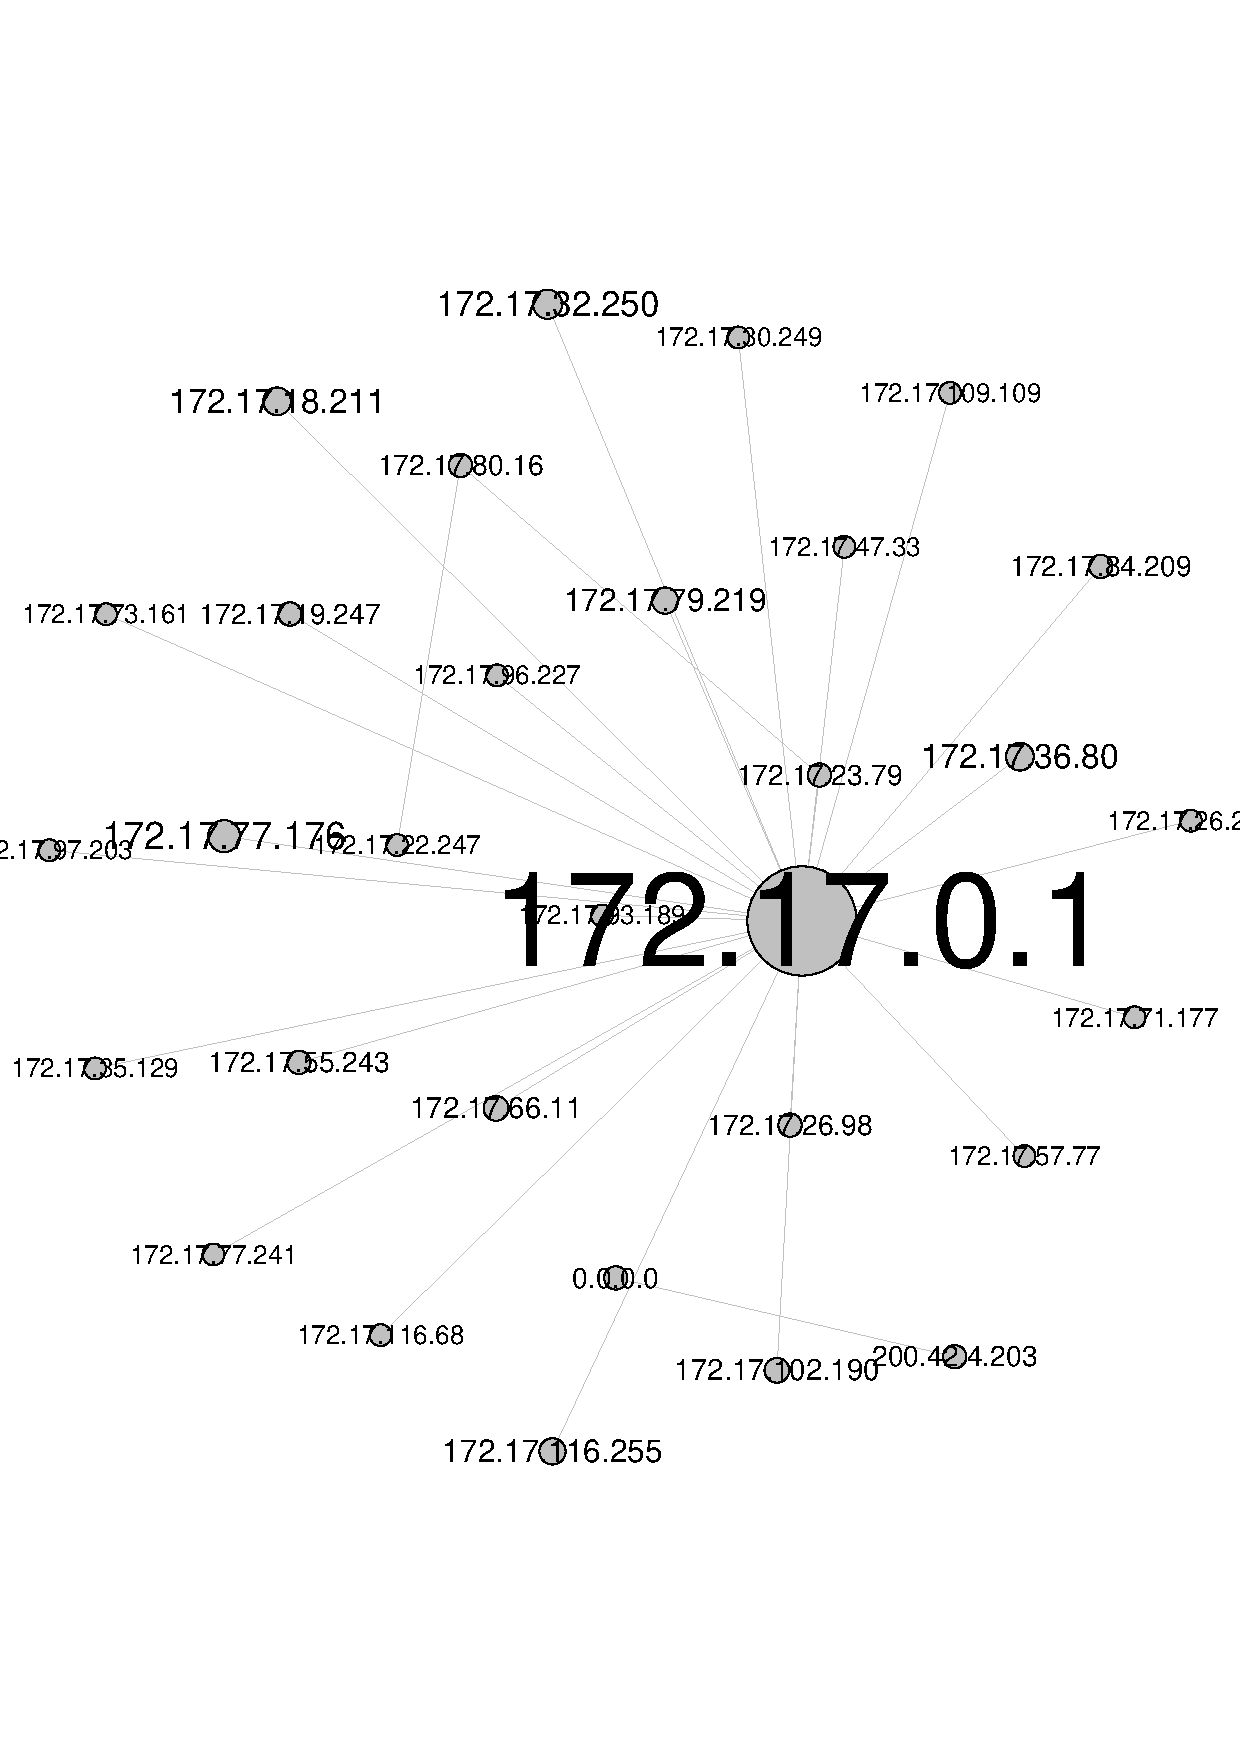
\includegraphics[scale=0.4]{figures/shopping.pdf}
	\caption{Red de mensajes \texttt{ARP} para captura del shopping.}
\end{figure}

\subsection{Escenario 3 (\emph{Starbucks})}

\begin{tikzpicture}[baseline]
    \begin{axis}[
            title={},
            xlabel={Símbolo (Dirección IP)},
            ylabel={Cantidad de información},
            scaled x ticks=false,
            scaled y ticks=false,
            width=0.45\textwidth,
            height=0.35\textwidth,
            legend pos=outer north east,
            legend cell align=left,
            ymin=0,
            xtick=data,
            xticklabels from table={../exp/starbucks.information}{IP},
            x tick label style={rotate=80,anchor=east,font=\small}
        ]
        \addplot [ybar, fill=blue!10, draw=blue] table[x=X-Pos,y=Information]
                {../exp/starbucks.information};

        \coordinate (A) at (axis cs:0,\StarbucksEntropy);
        \coordinate (O1) at (rel axis cs:0,0);
        \coordinate (O2) at (rel axis cs:1,0);

        \draw [blue, thick] (A -| O1) -- (A -| O2);

    \end{axis}
\end{tikzpicture}

\begin{figure}[H]
	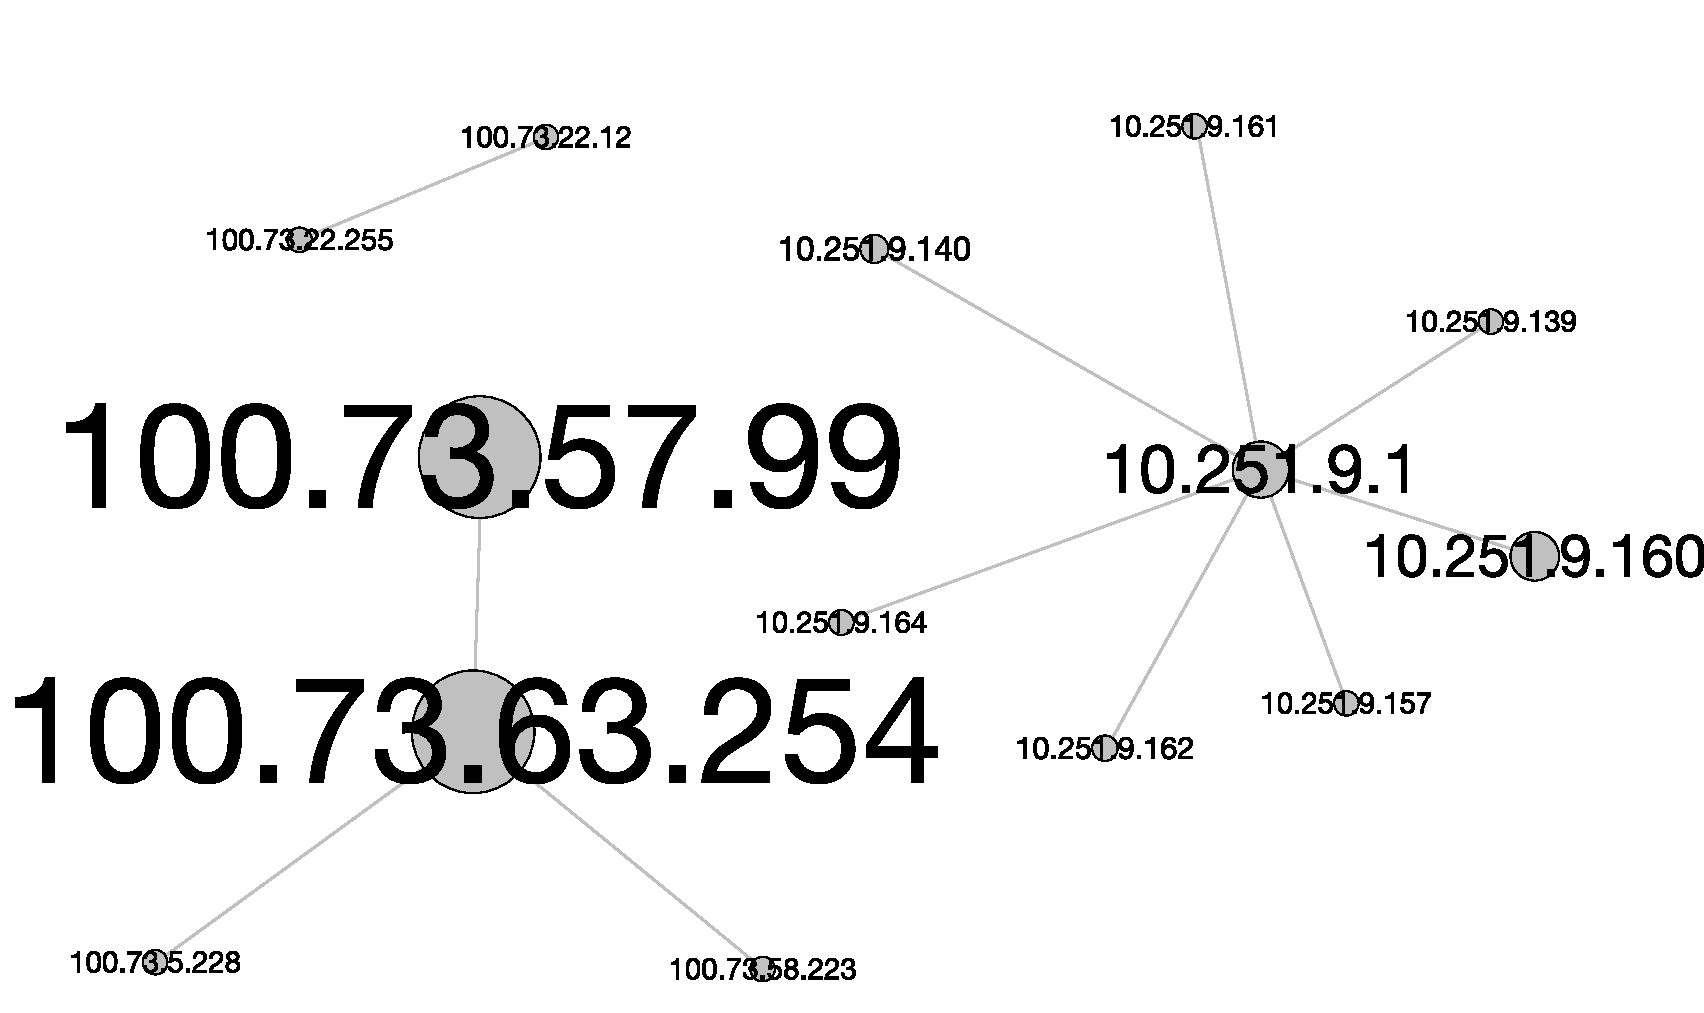
\includegraphics[scale=0.4]{figures/starbucks.pdf}
	\caption{Red de mensajes \texttt{ARP} para captura del Starbucks.}
\end{figure}
